\section*{\Large\centering \textbf{APPENDIX}}
\addcontentsline{toc}{section}{APPENDIX}

\begin{table}[h!]
    \centering
    \caption{Meeting log with supervisor detailing project discussions and feedback.}
    \begin{tabularx}{\textwidth}{|c|c|c|X|}
        \hline
        \textbf{Date} & \textbf{Time} & \textbf{Purpose of Visit}   & \textbf{Discussion / Notes}                                                                                                                         \\
        \hline
        2025-05-15    & 11:00 AM      & Project proposal discussion & Discussed scope and objectives of the UrbanFix project. Supervisor suggested including analytics and leaderboard features.                          \\
        \hline
        2025-06-05    & 1:30 PM       & UI and functionality review & Reviewed My Reports page and notifications implementation. Supervisor approved current design; suggested minor improvements in map visualization.   \\
        \hline
        2025-06-27    & 11:00 AM      & Backend logic discussion    & Discussed analytics data aggregation and leaderboard calculation. Supervisor advised implementing resolution rate and category-wise statistics.     \\
        \hline
        2025-07-24    & 11:00 AM      & Testing and validation      & Demonstrated in-app notifications, analytics graphs, and leaderboard. Supervisor provided feedback on edge cases and recommended adding unit tests. \\
        \hline
        2025-09-23    & 1:30 PM       & Final review                & Reviewed full project functionality including maps, analytics, notifications, and leaderboard. Supervisor approved for report submission.           \\
        \hline
    \end{tabularx}
\end{table}

\begin{figure}[H]
    \centering
    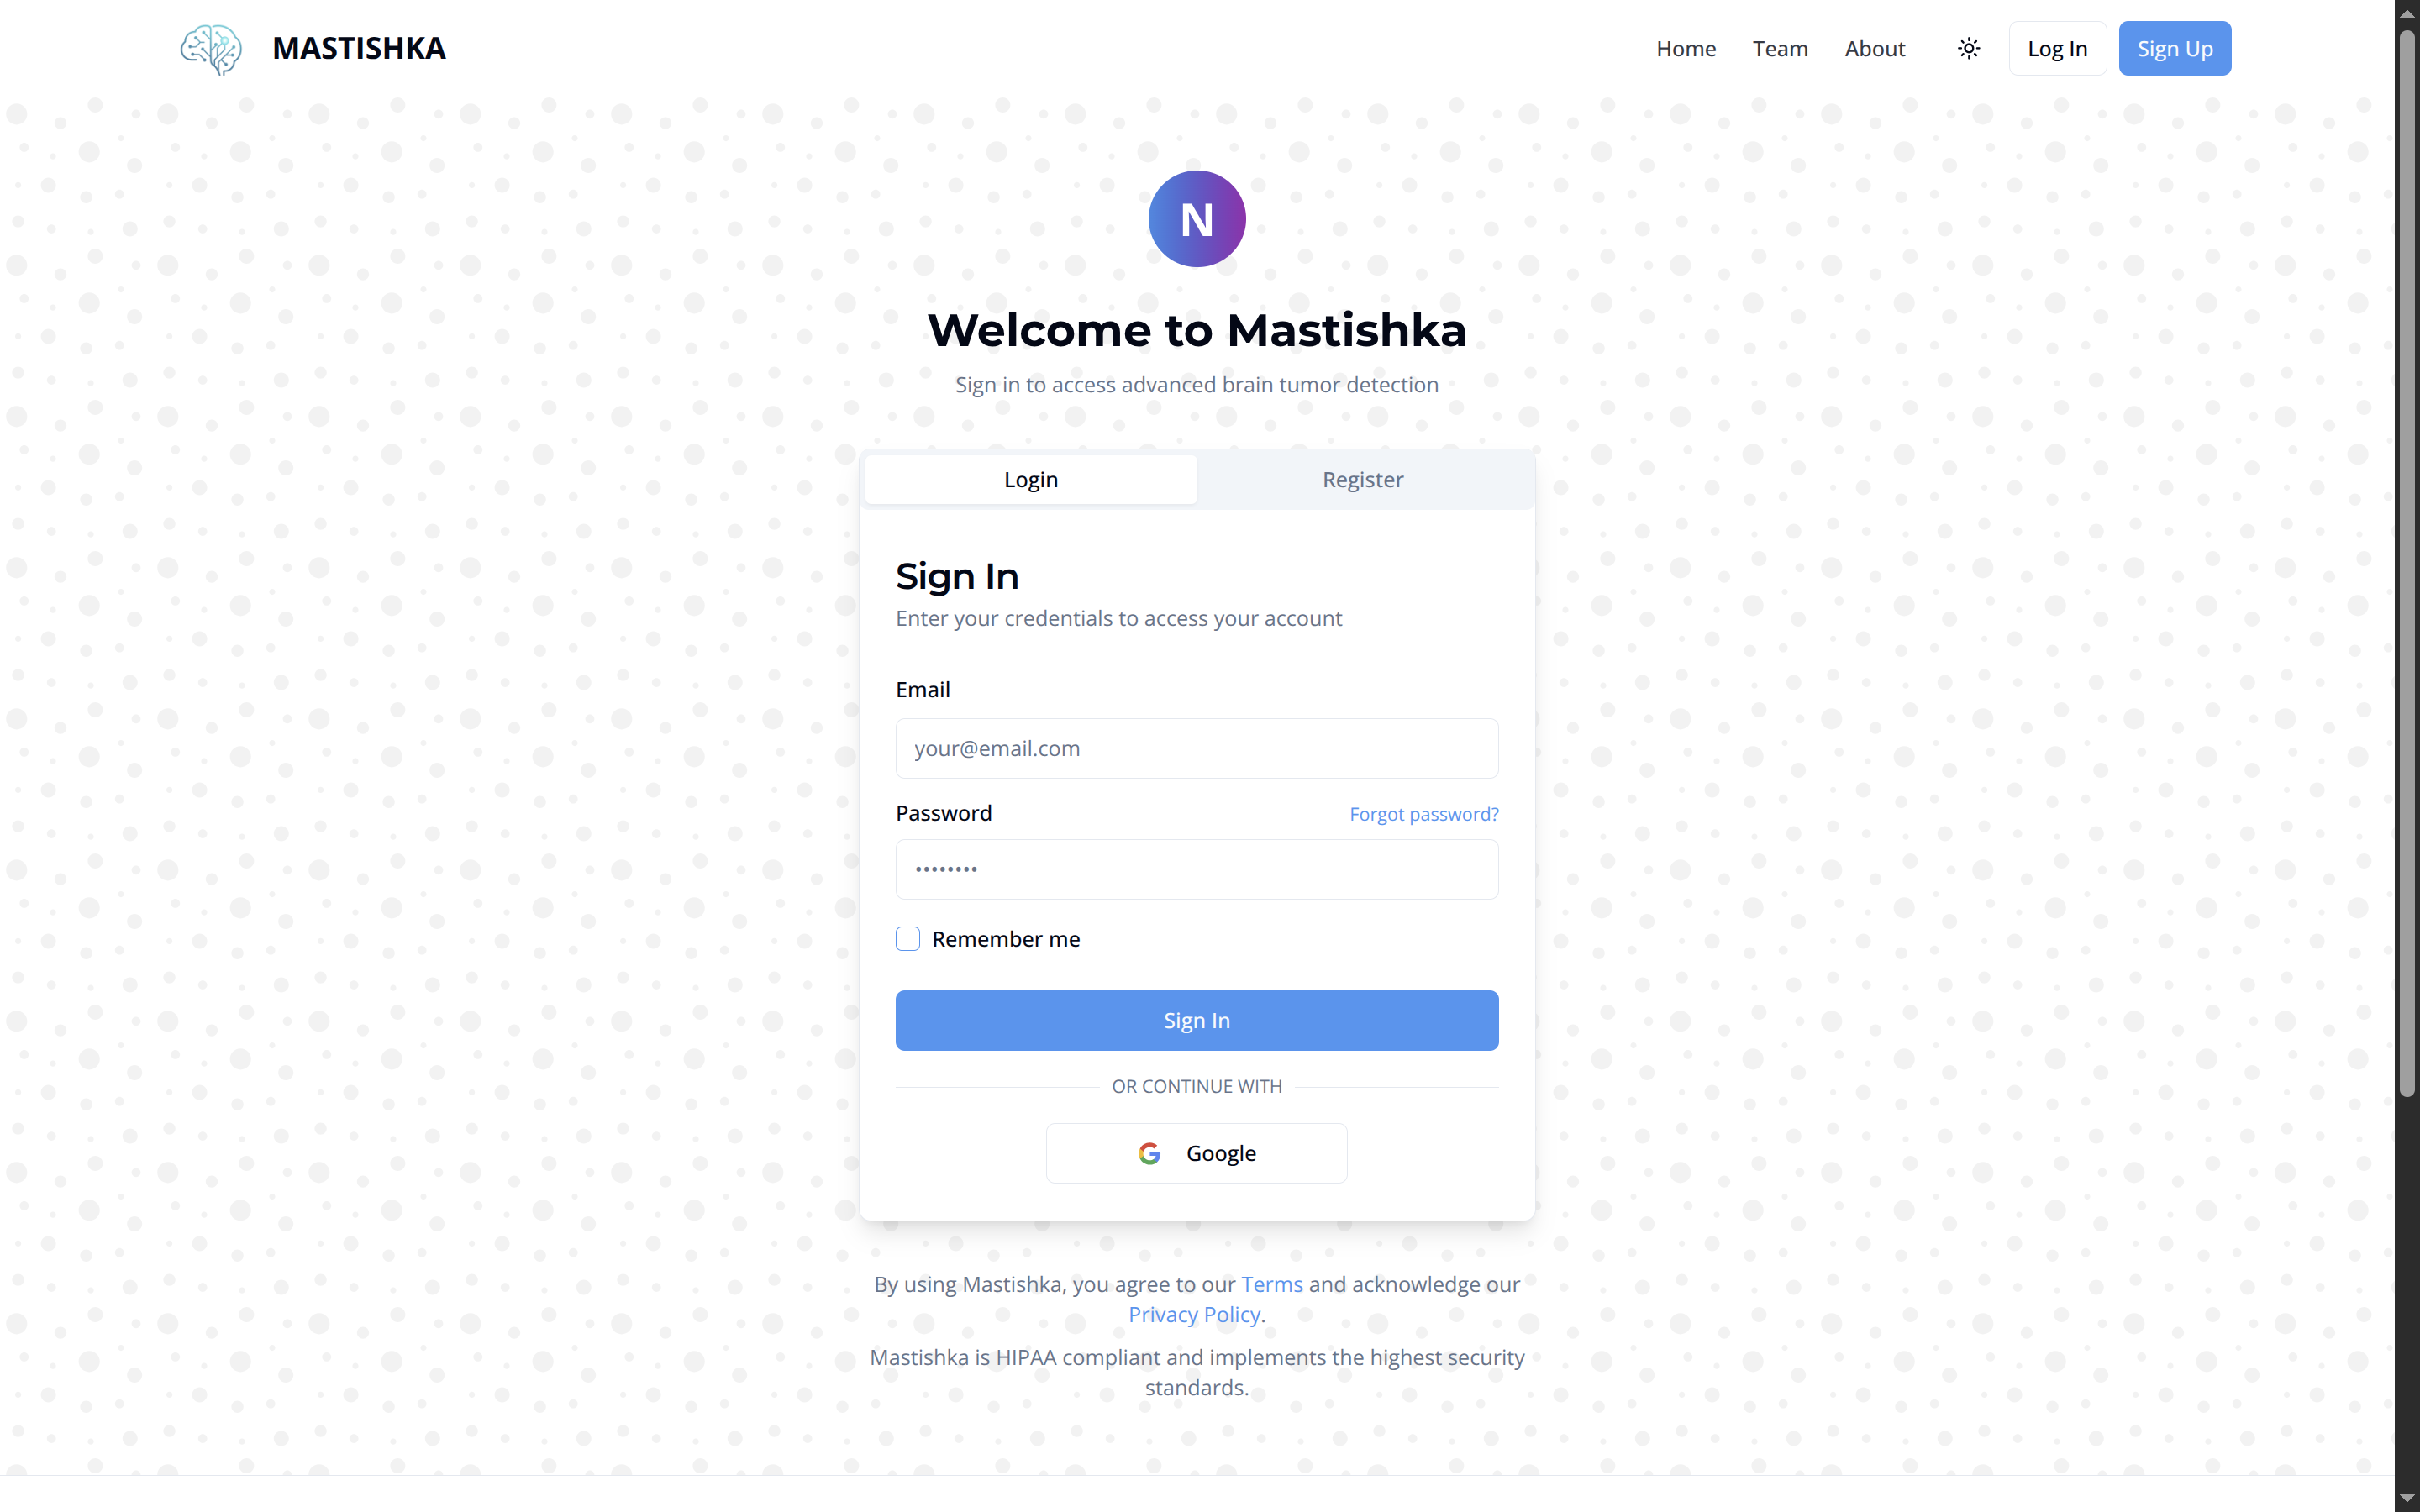
\includegraphics[width=1\linewidth]{App/login.png}
    \caption{Login page of the web application}
    \label{fig:login_page}
\end{figure}

\begin{figure}[H]
    \centering
    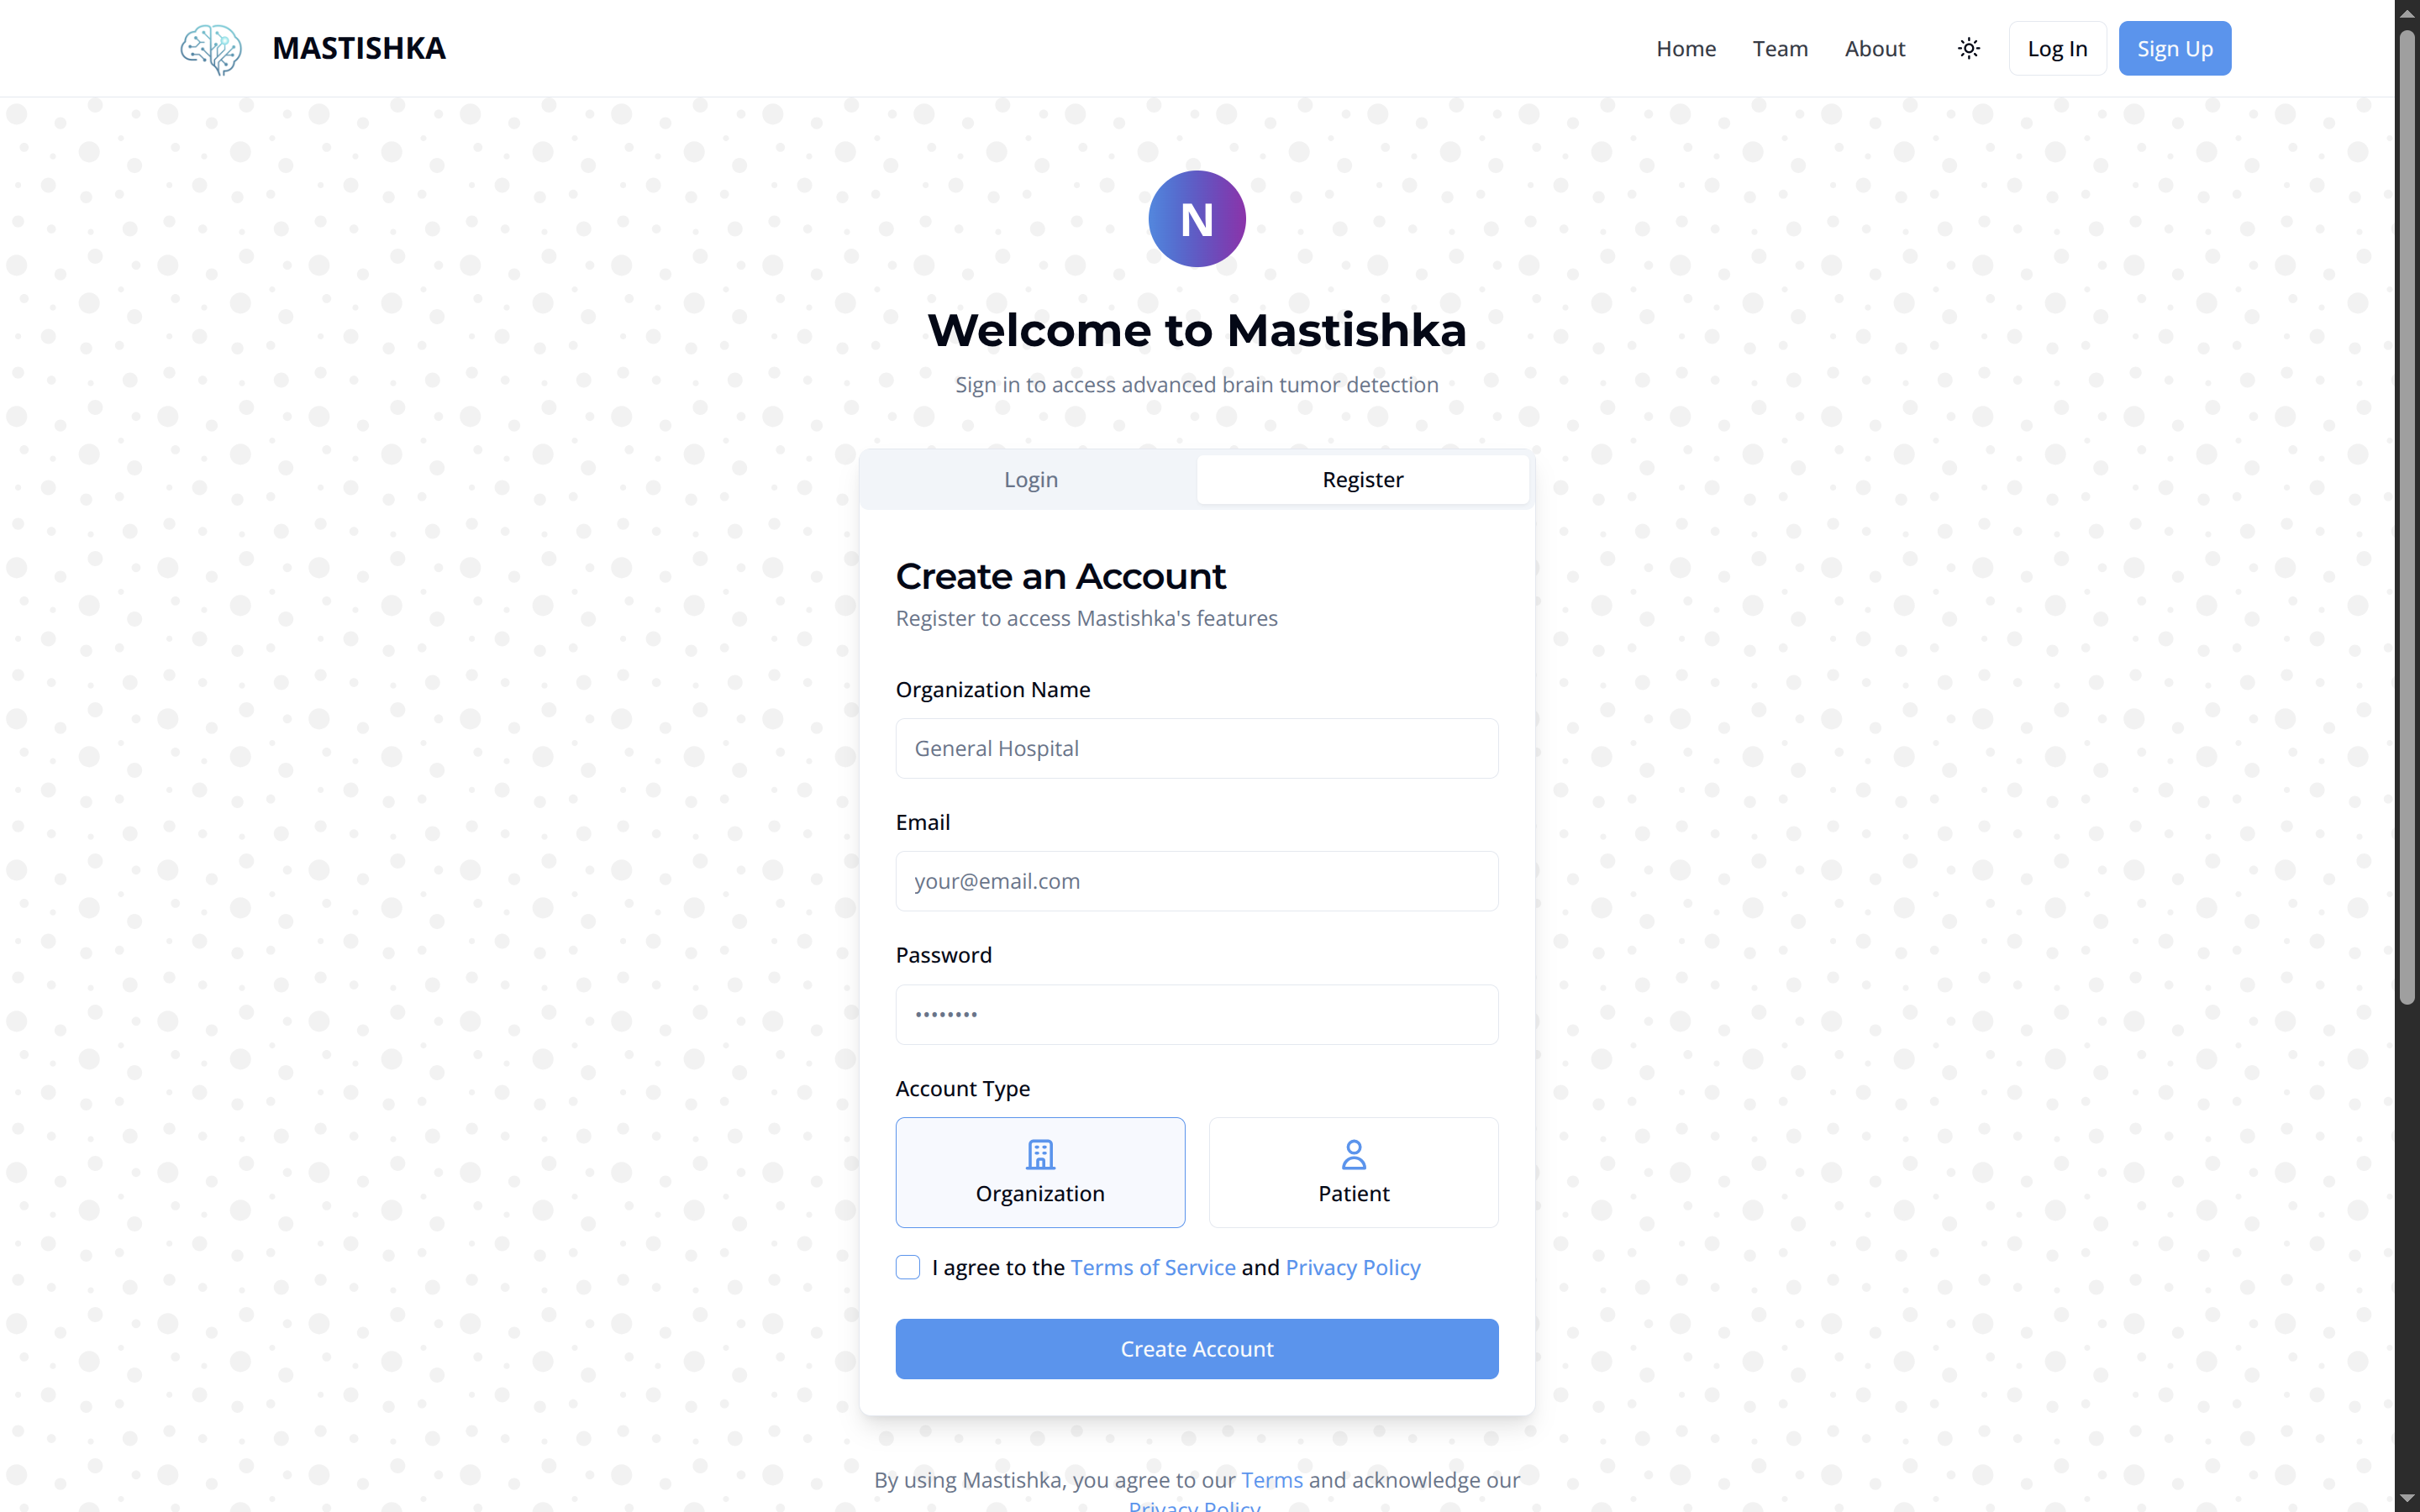
\includegraphics[width=1\linewidth]{App/signin.png}
    \caption{Sign in page of the web application}
    \label{fig:signin_page}
\end{figure}

\begin{figure}[H]
    \centering
    
\includegraphics[width=0.8\linewidth]{App/home.png}
    \caption{Home page of the web application}
    \label{fig:home_page}
\end{figure}

\begin{figure}[H]
    \centering
    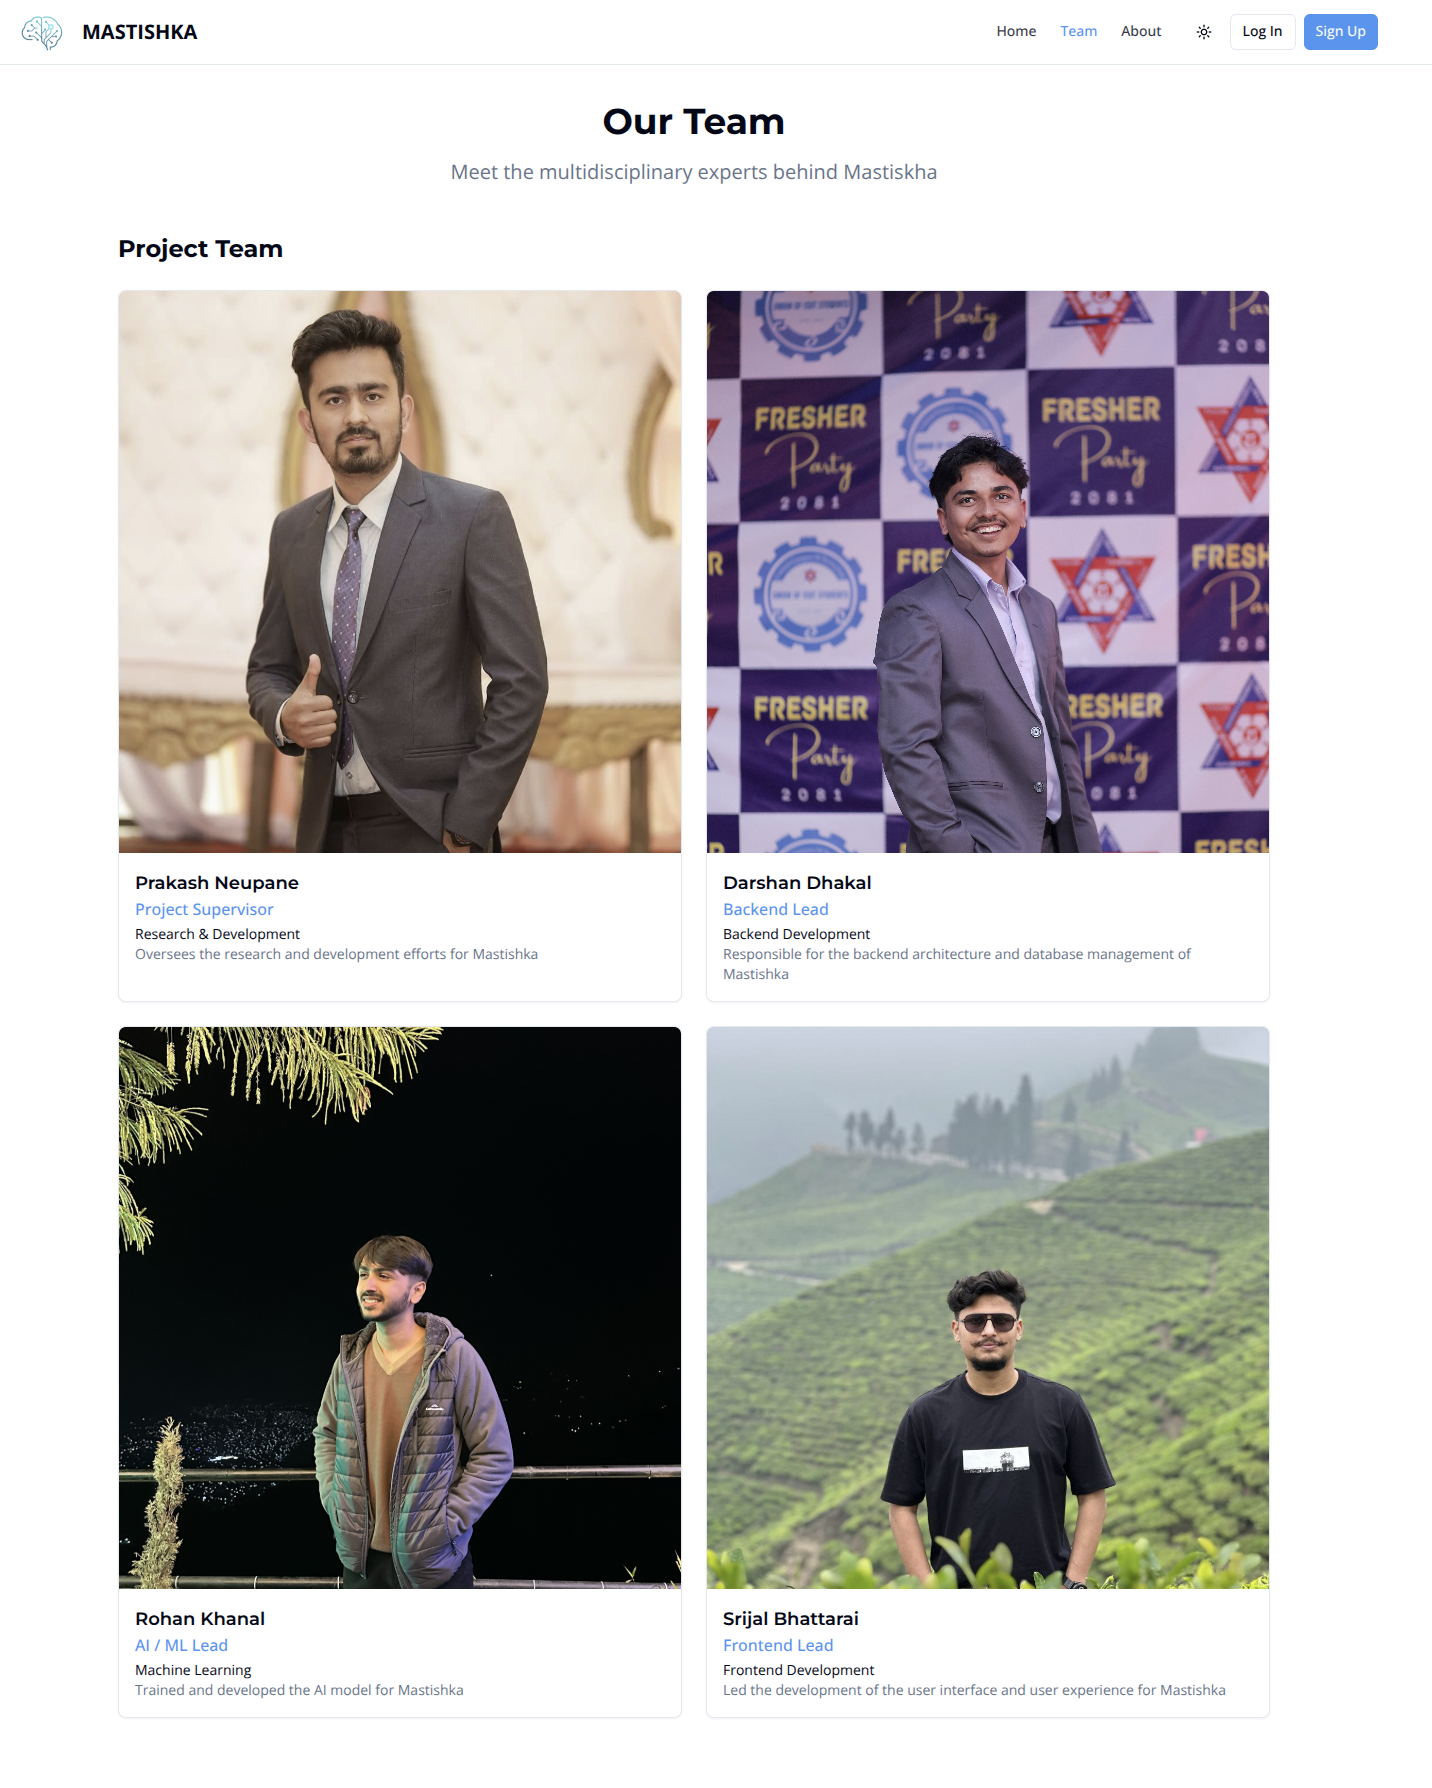
\includegraphics[width=0.7\linewidth]{App/team.png}
    \caption{Team page of the web application}
    \label{fig:team_page}
\end{figure}

\begin{figure}[H]
    \centering
    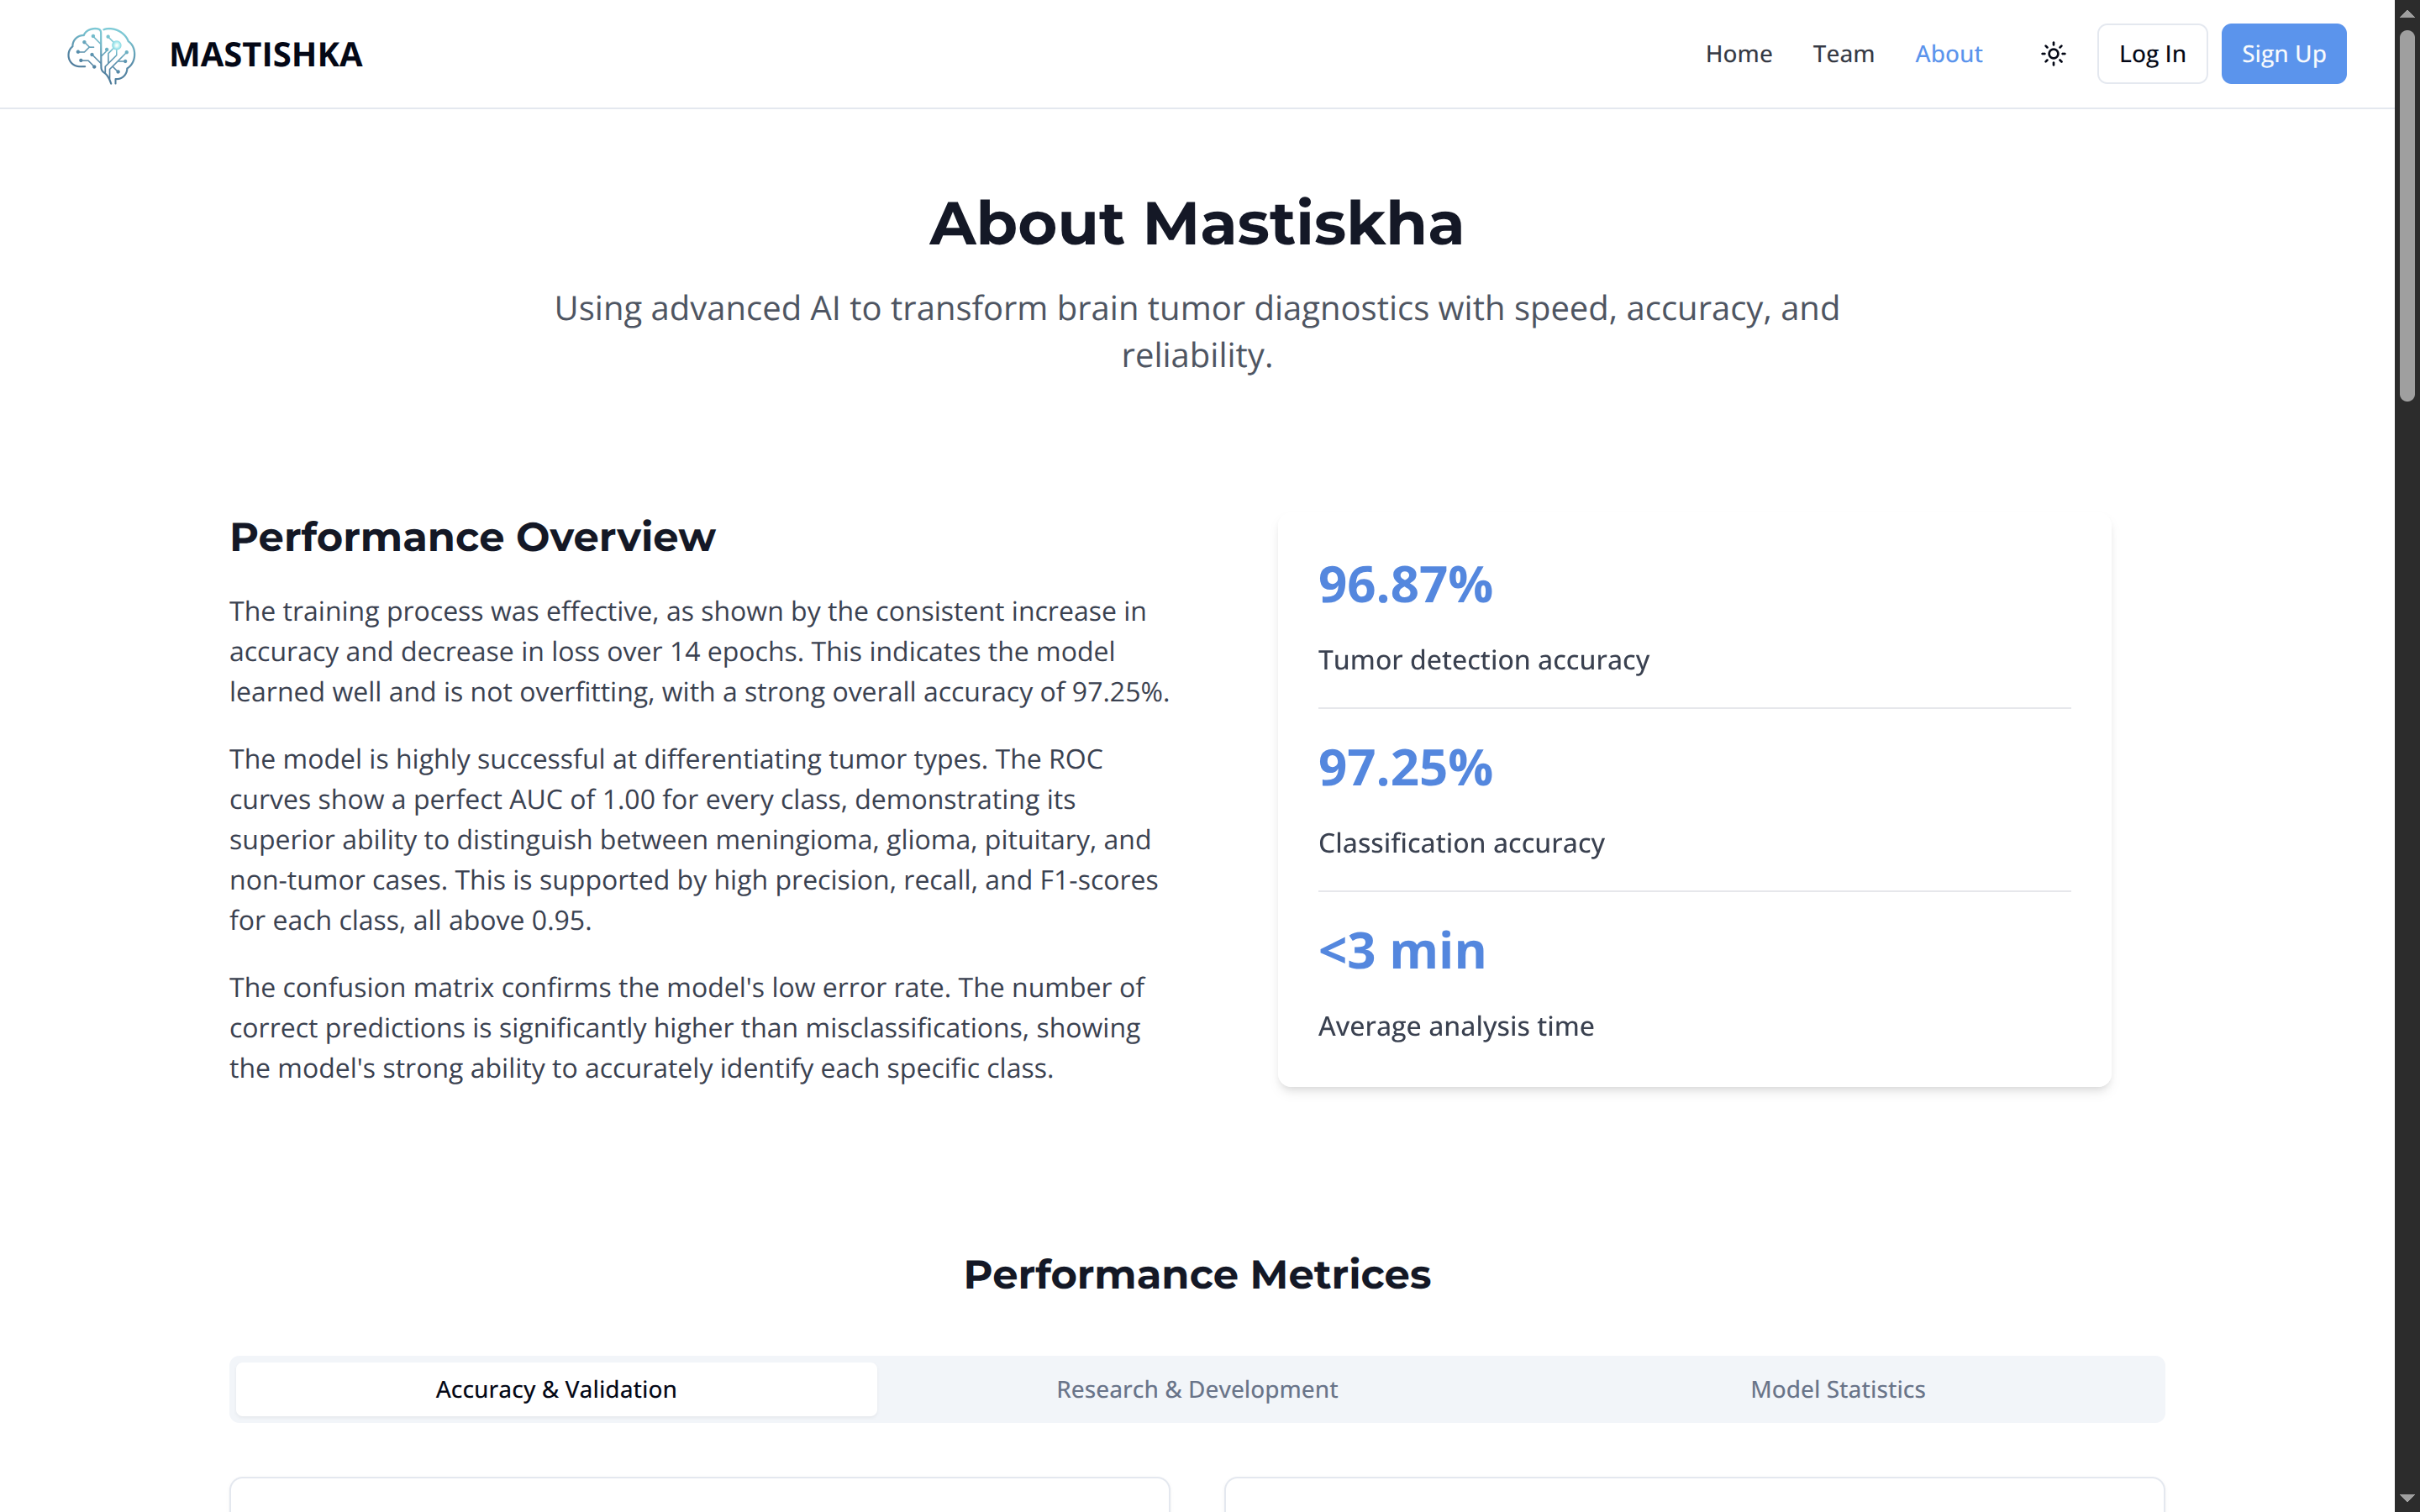
\includegraphics[width=1\linewidth]{App/stats.png}
    \caption{Statistics page of the web application}
    \label{fig:stats_page}
\end{figure}

\begin{figure}[H]
    \centering
    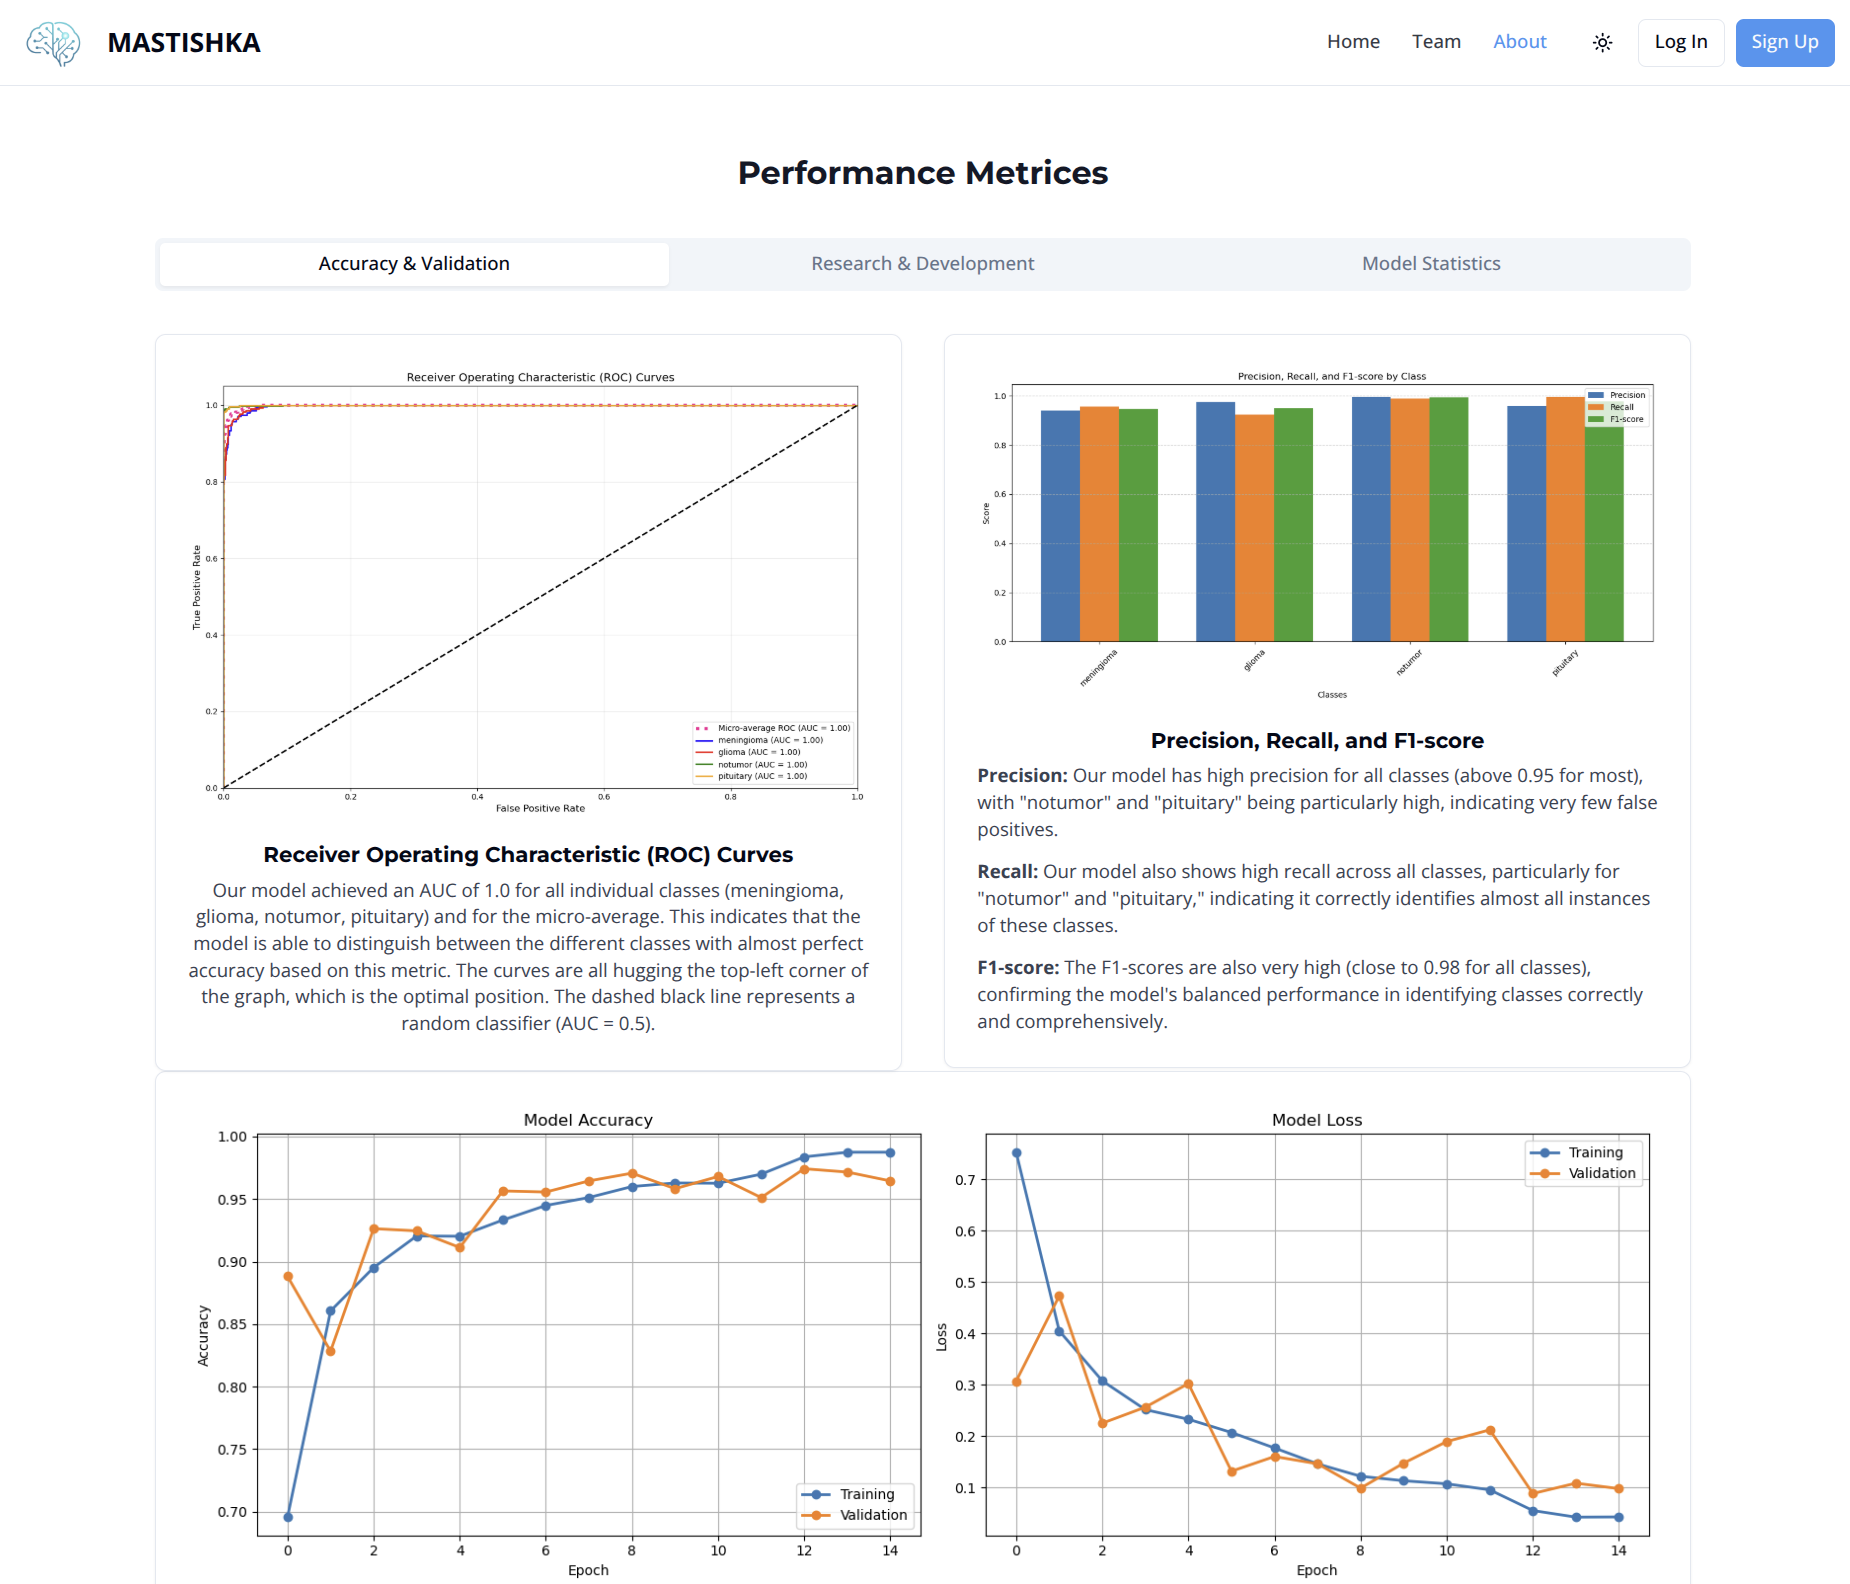
\includegraphics[width=0.8\linewidth]{App/stats2.png}
    \caption{Statistics page of the web application}
    \label{fig:stats2_page}
\end{figure}

\begin{figure}[H]
    \centering
    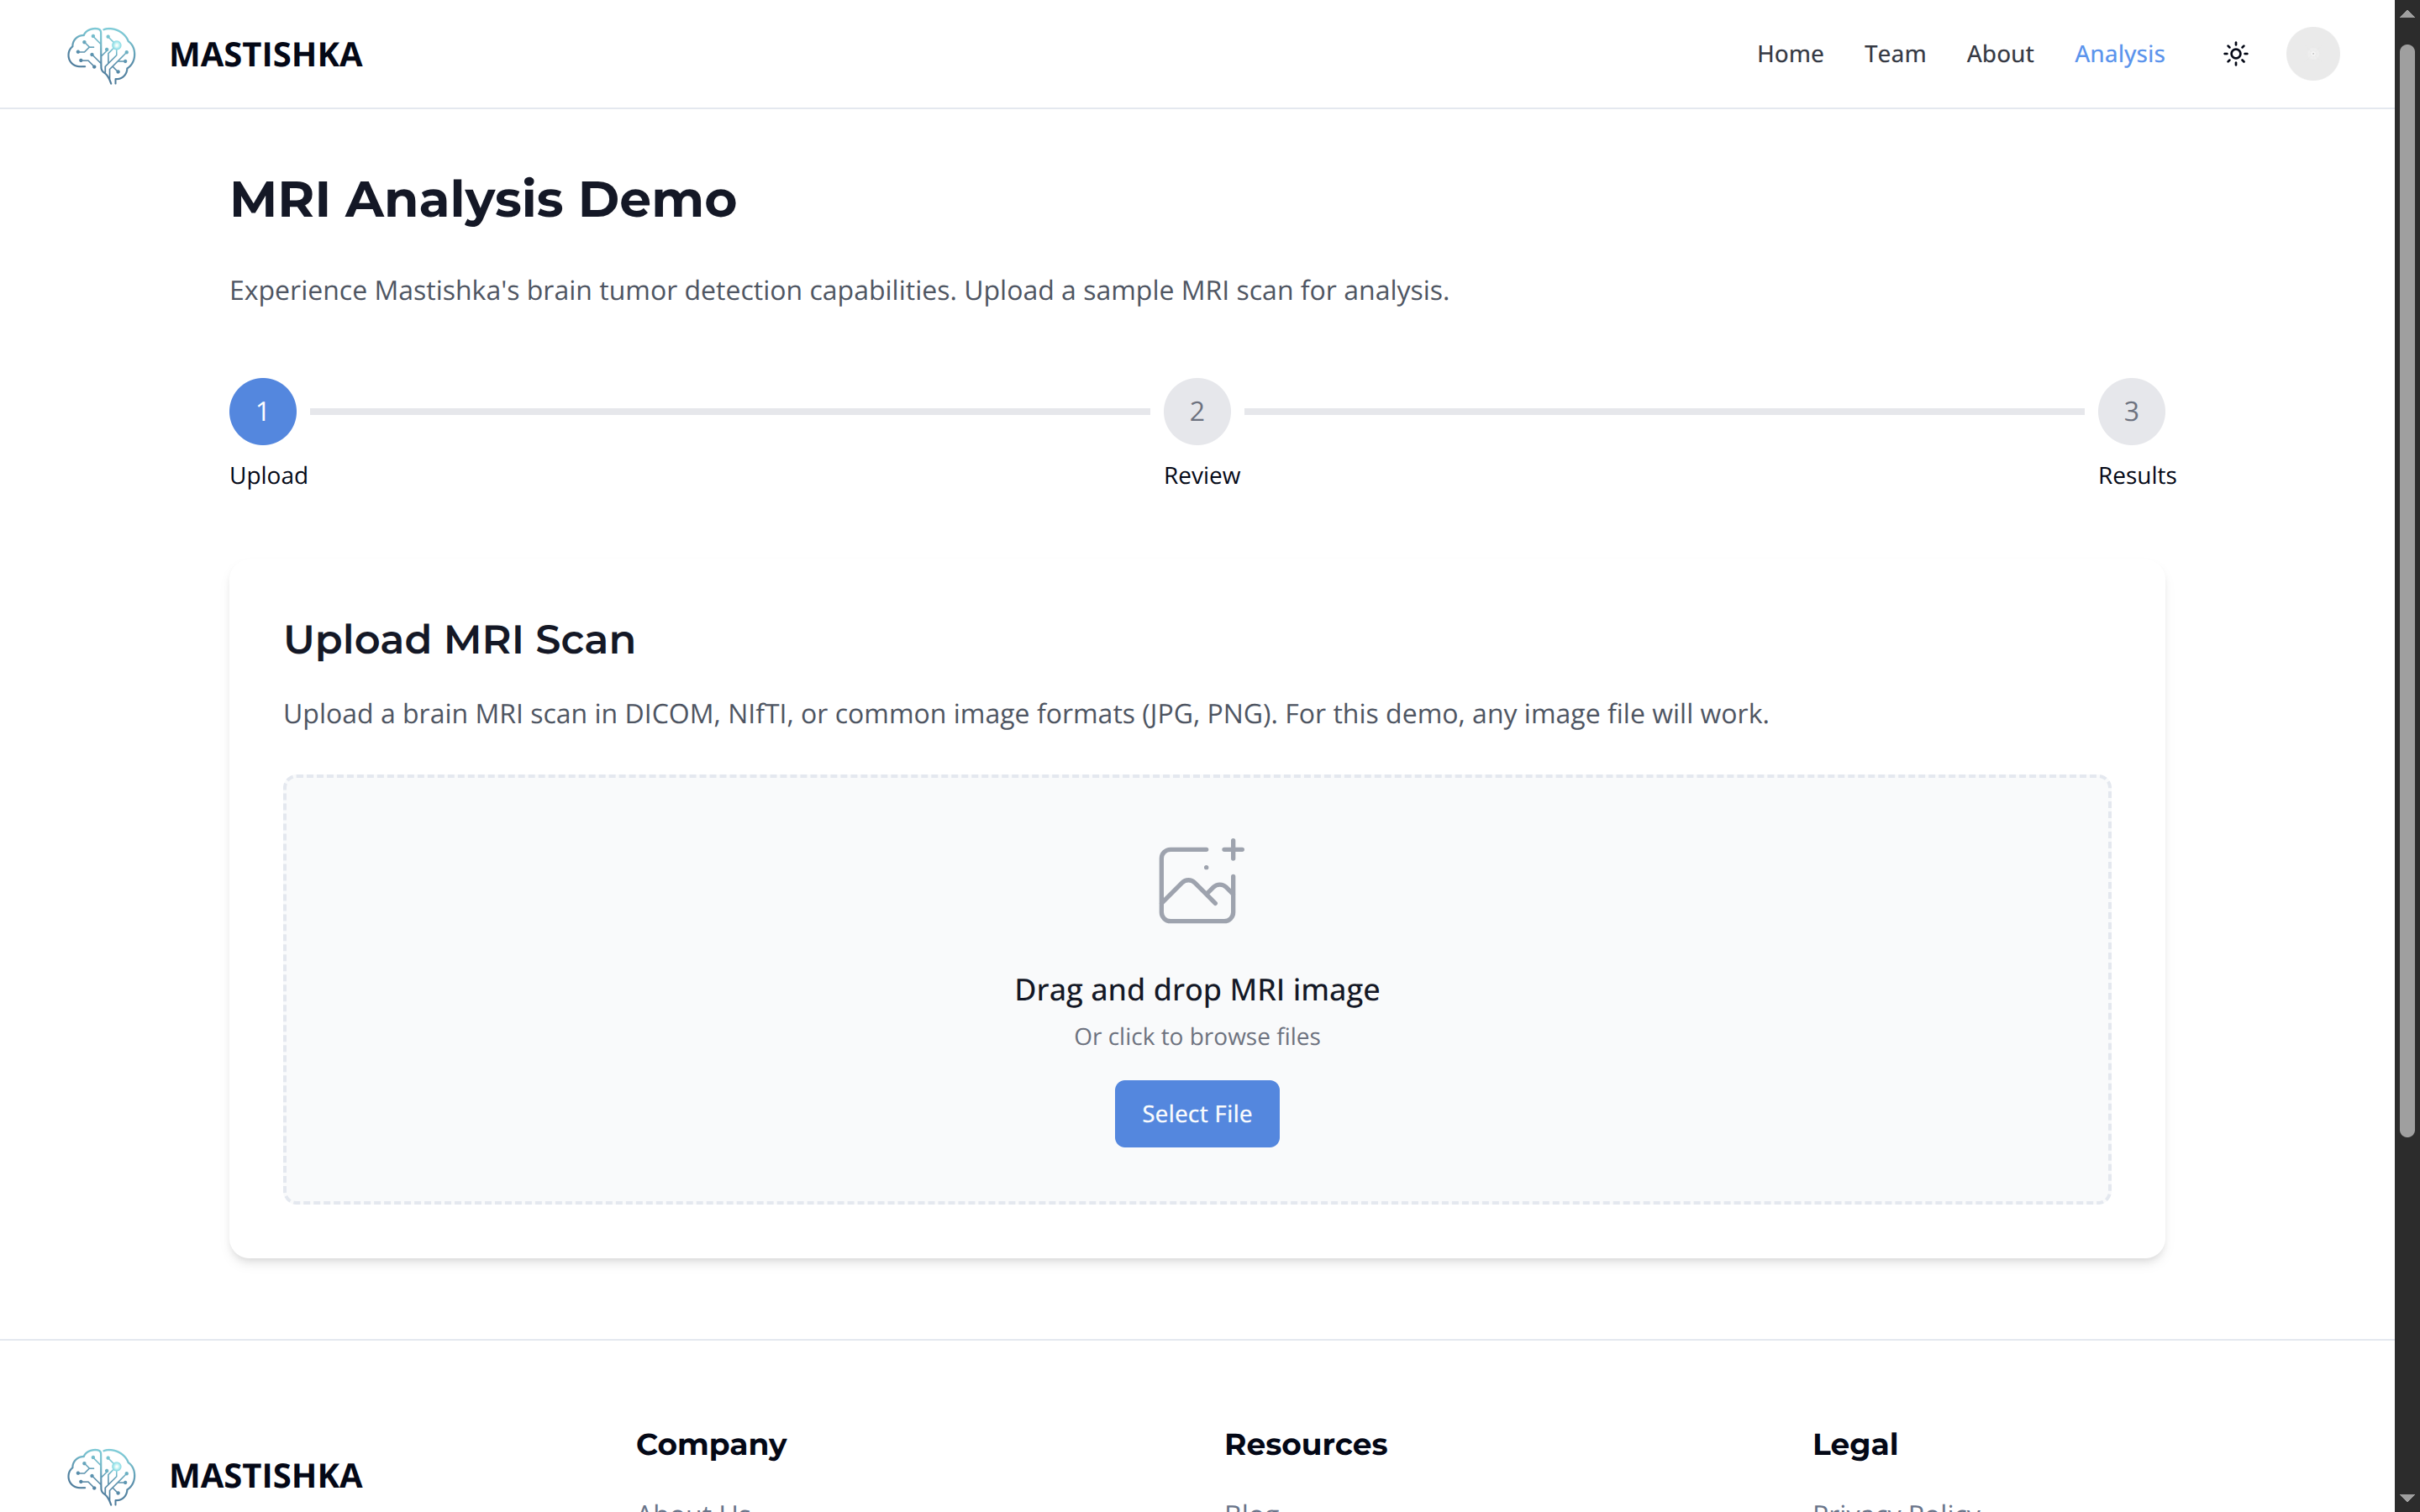
\includegraphics[width=0.9\linewidth]{App/analysis.png}
    \caption{Analysis page of the web application}
    \label{fig:analysis_page}
\end{figure}

\begin{figure}[H]
    \centering
    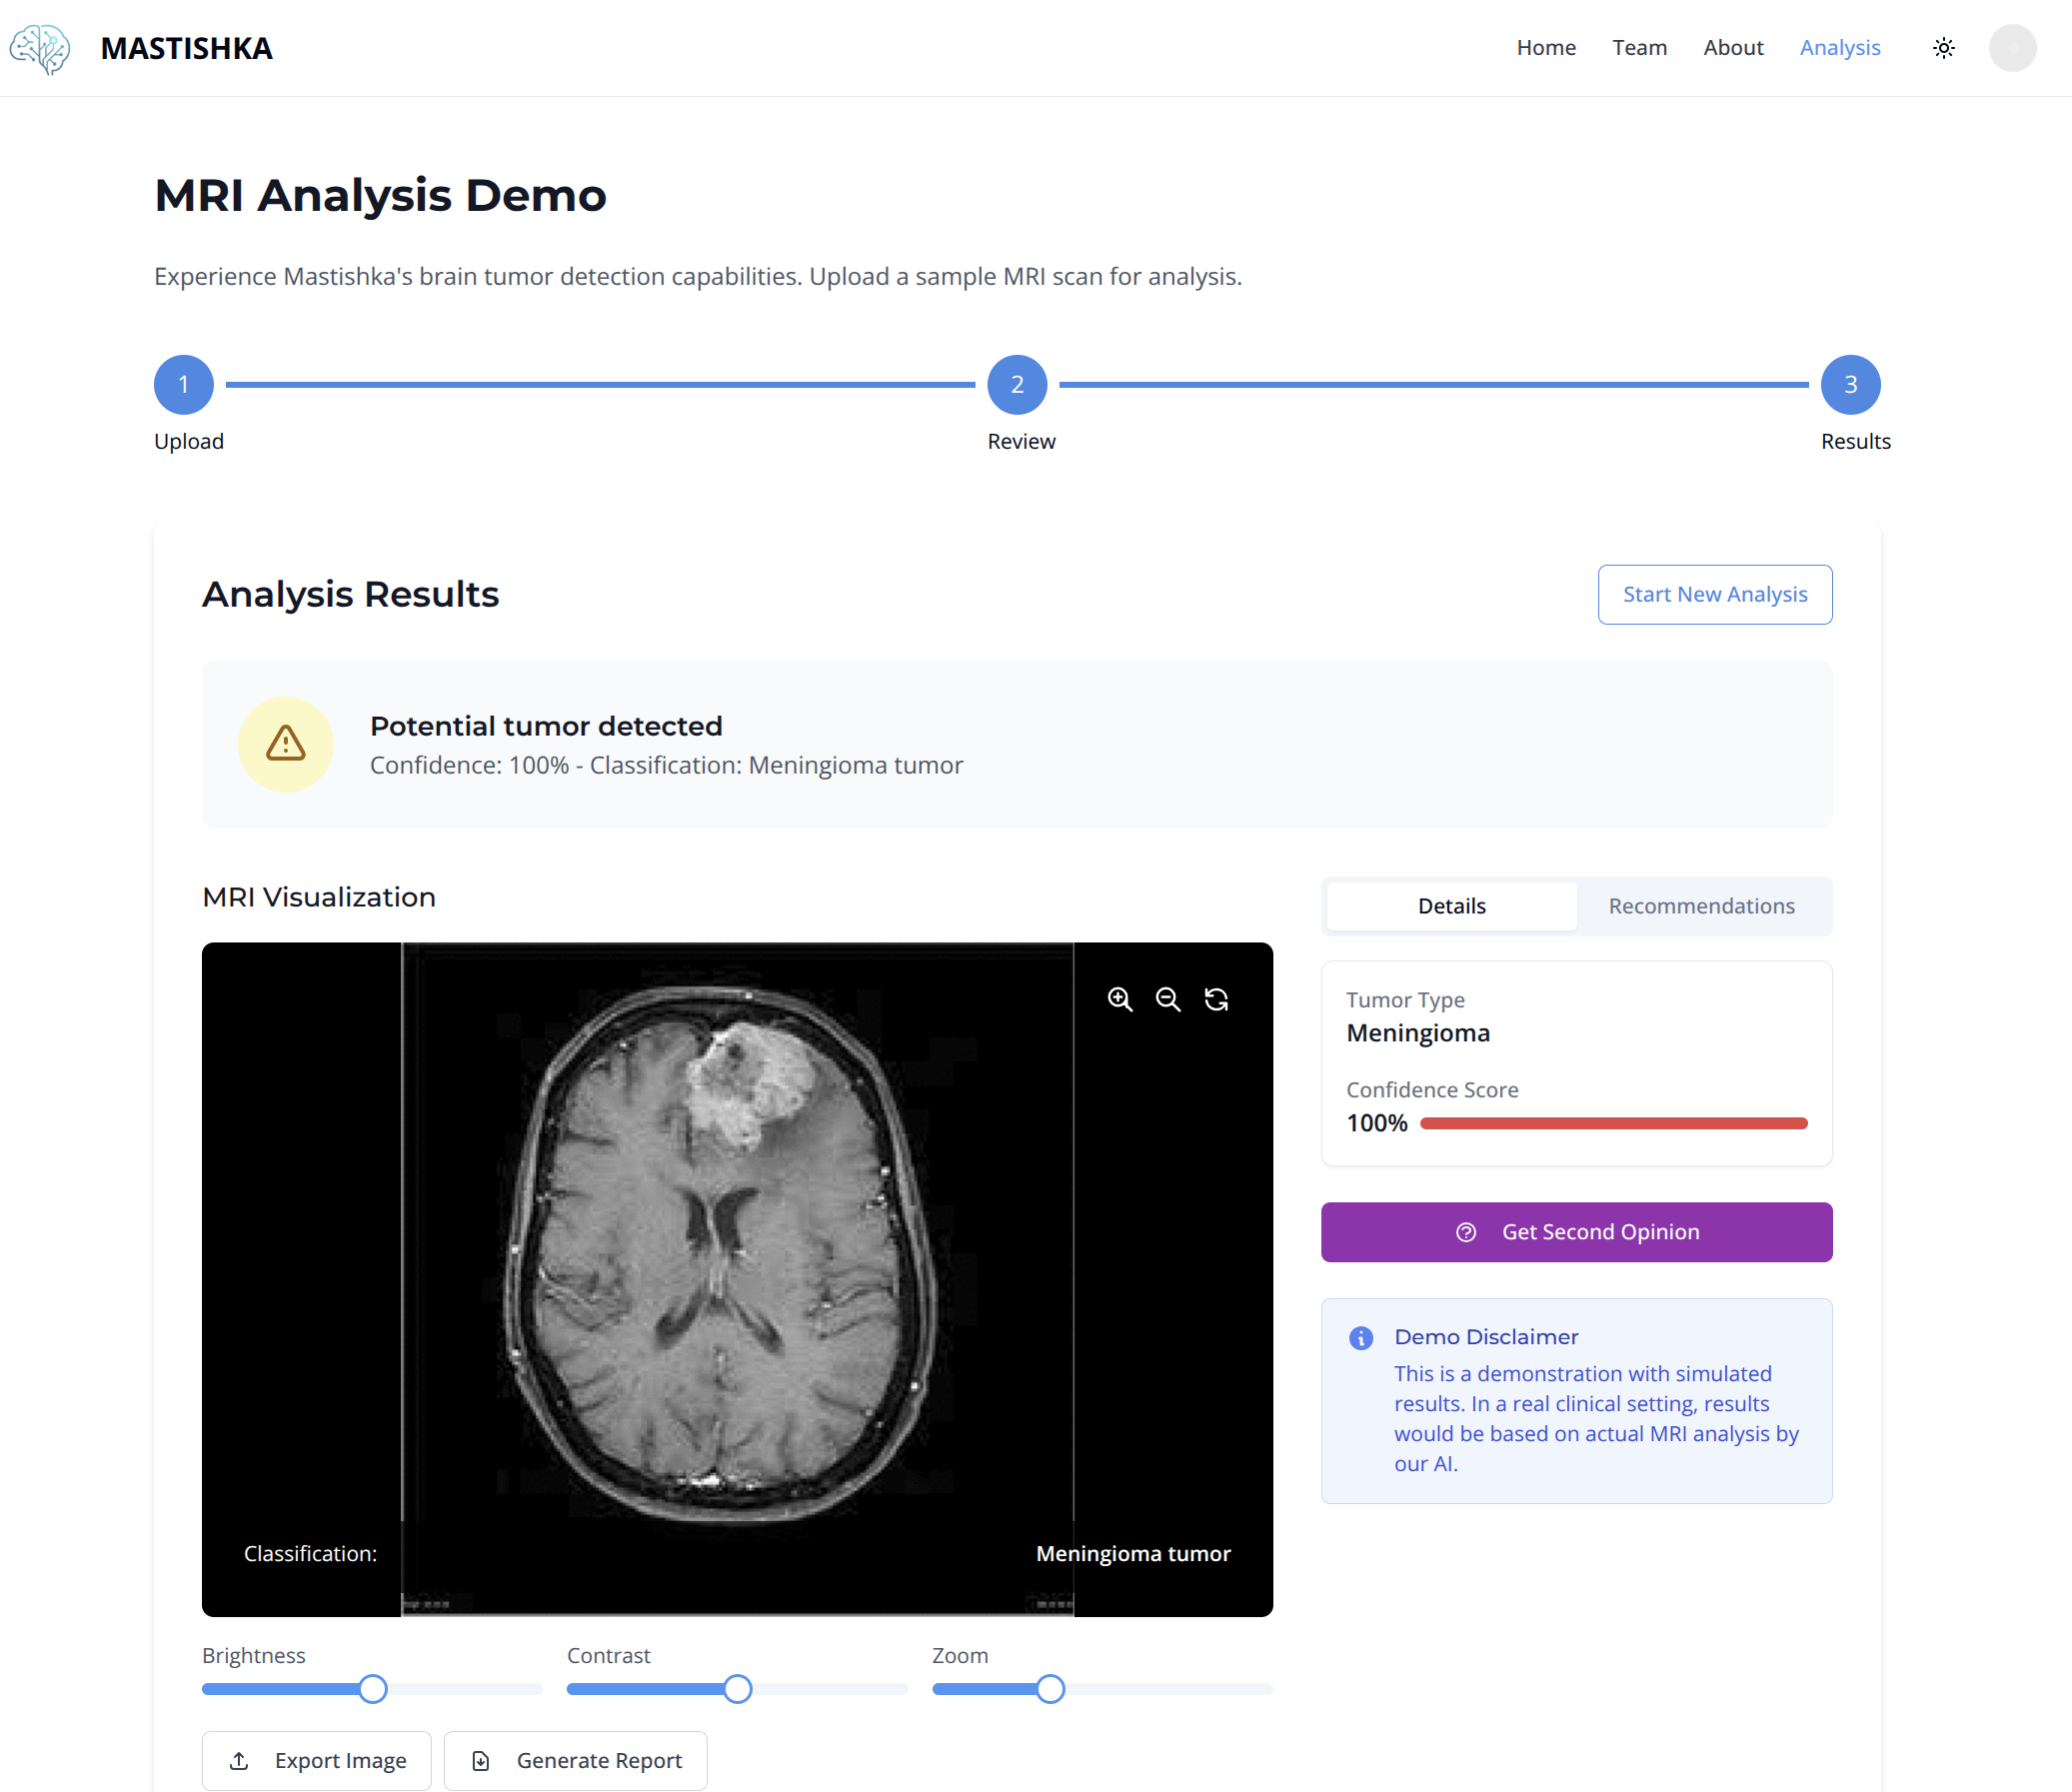
\includegraphics[width=1\linewidth]{App/analysis2.png}
    \caption{Analysis page of the web application}
    \label{fig:analysis2_page}
\end{figure}

\begin{figure}[H]
    \centering
    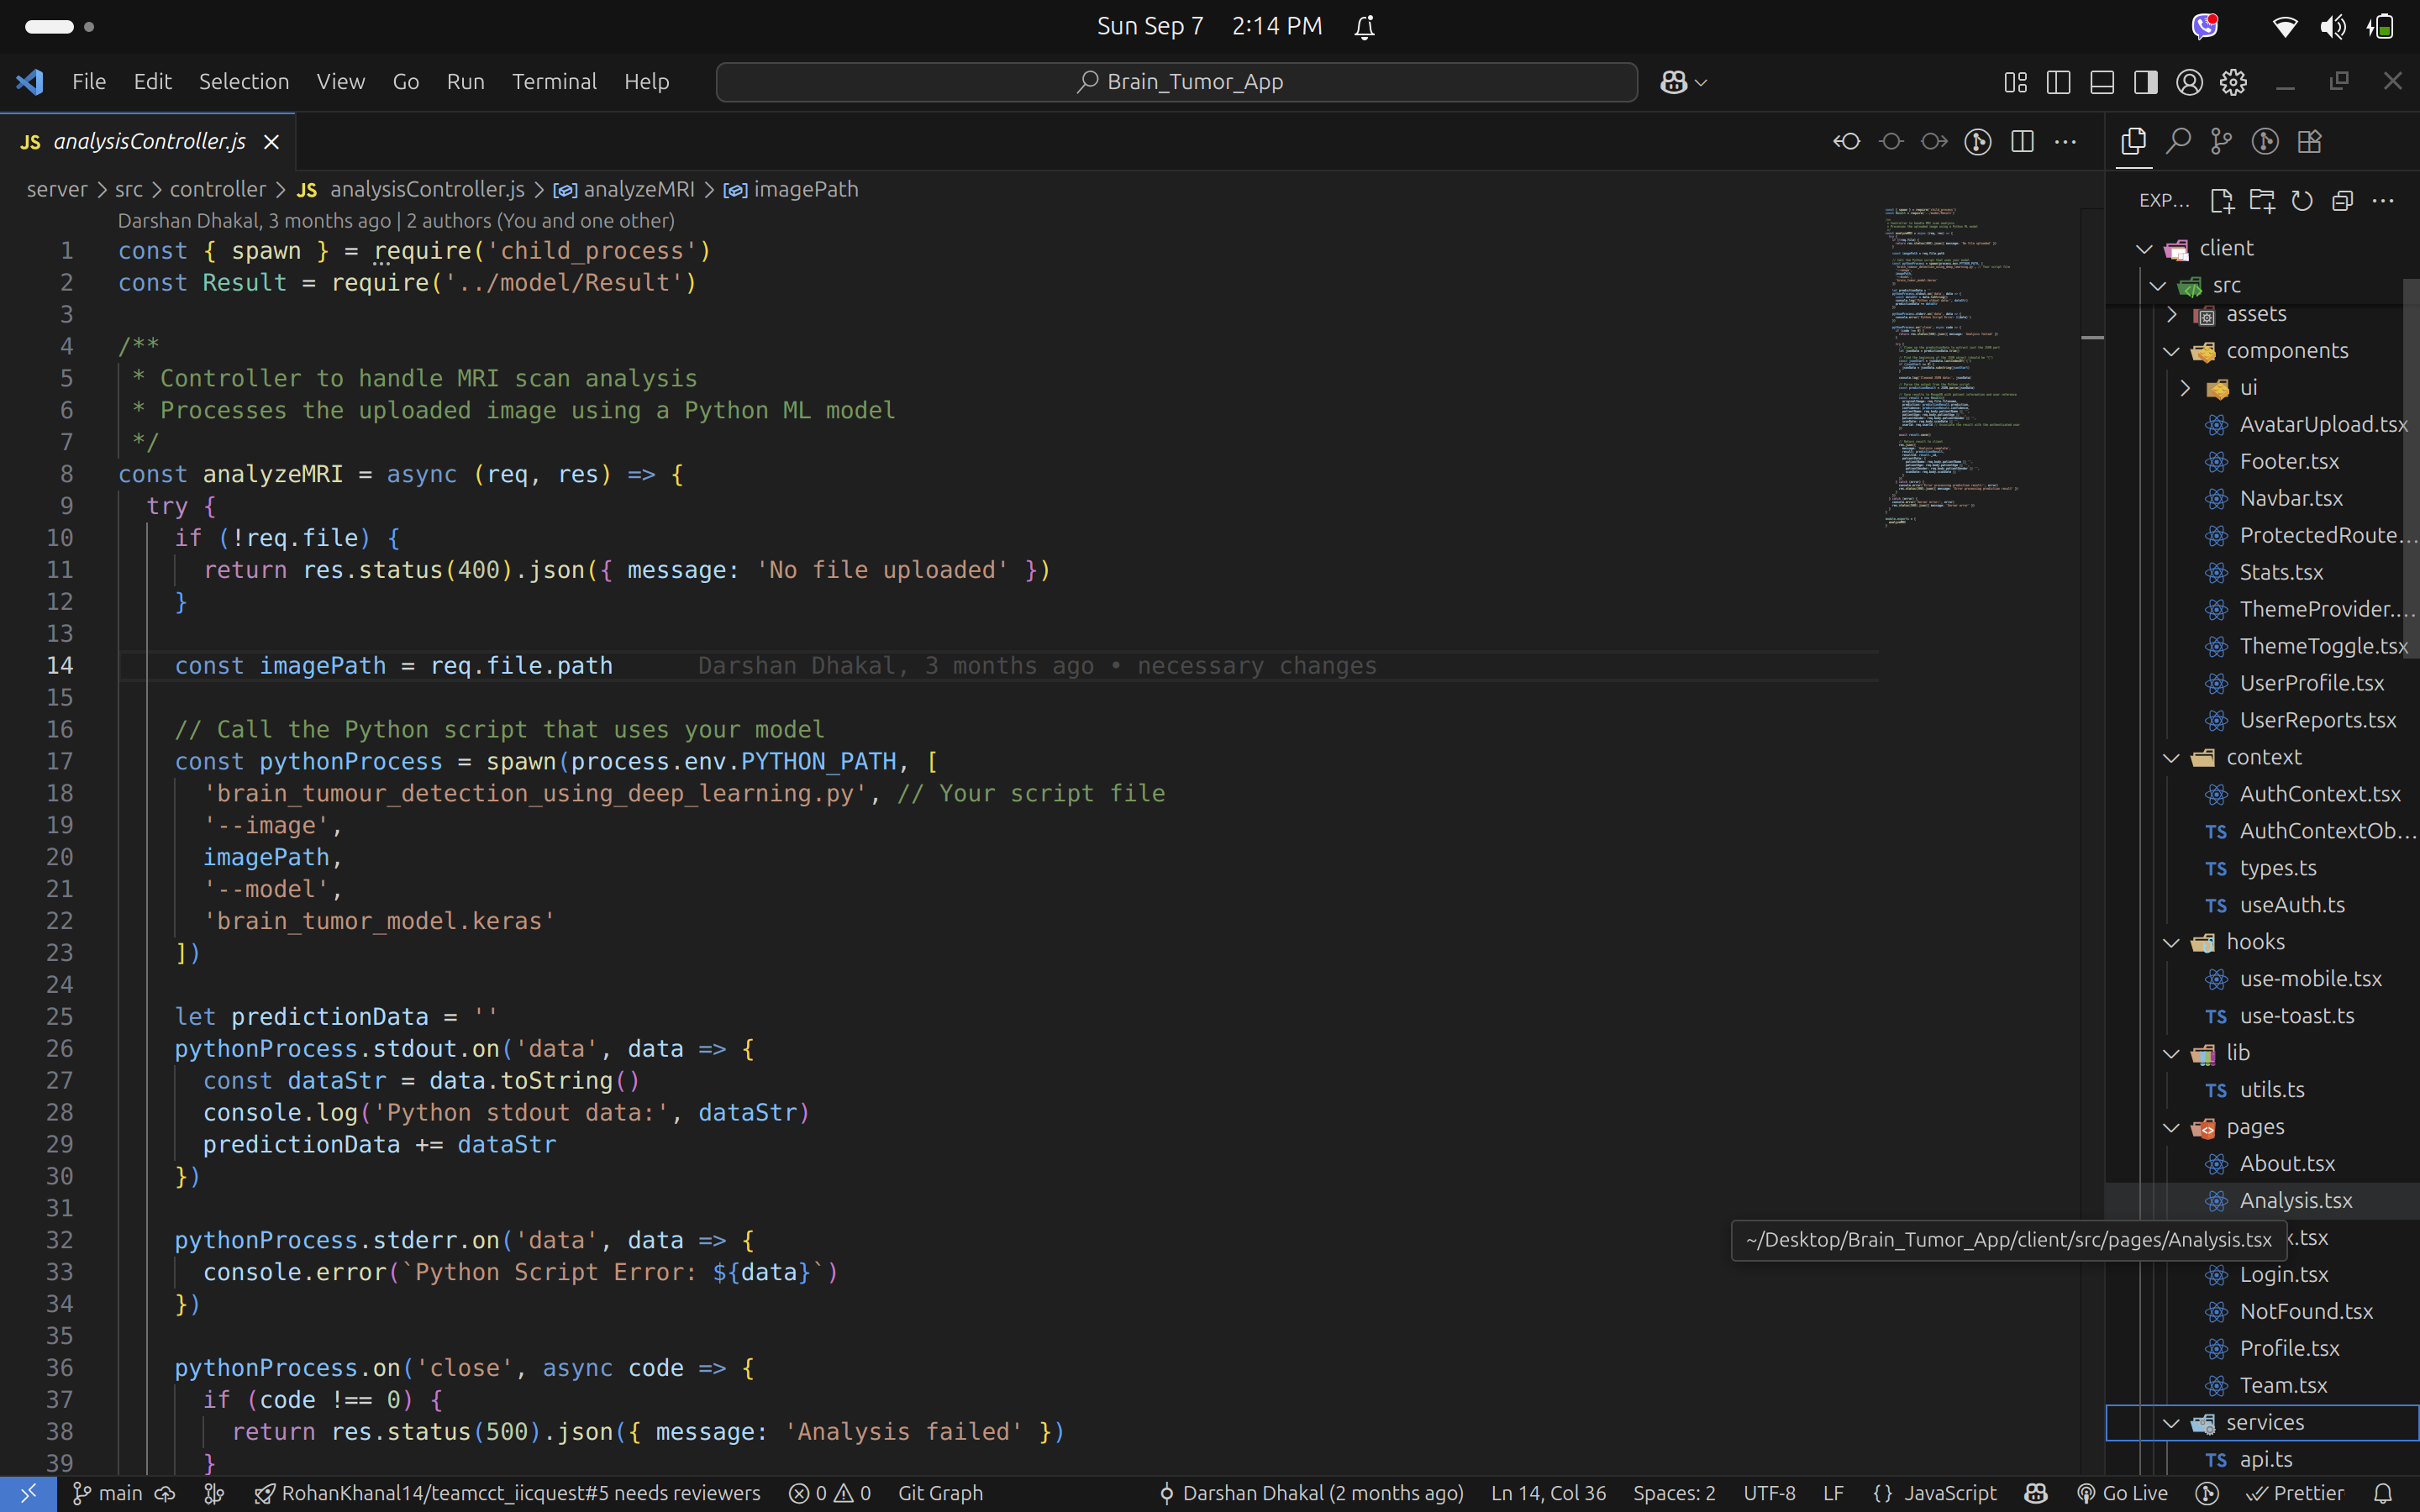
\includegraphics[width=1\linewidth]{App/Frontend.png}
    \caption{Frontend File Structure of the web application}
    \label{fig:frontend_page}
\end{figure}

\begin{figure}[H]
    \centering
    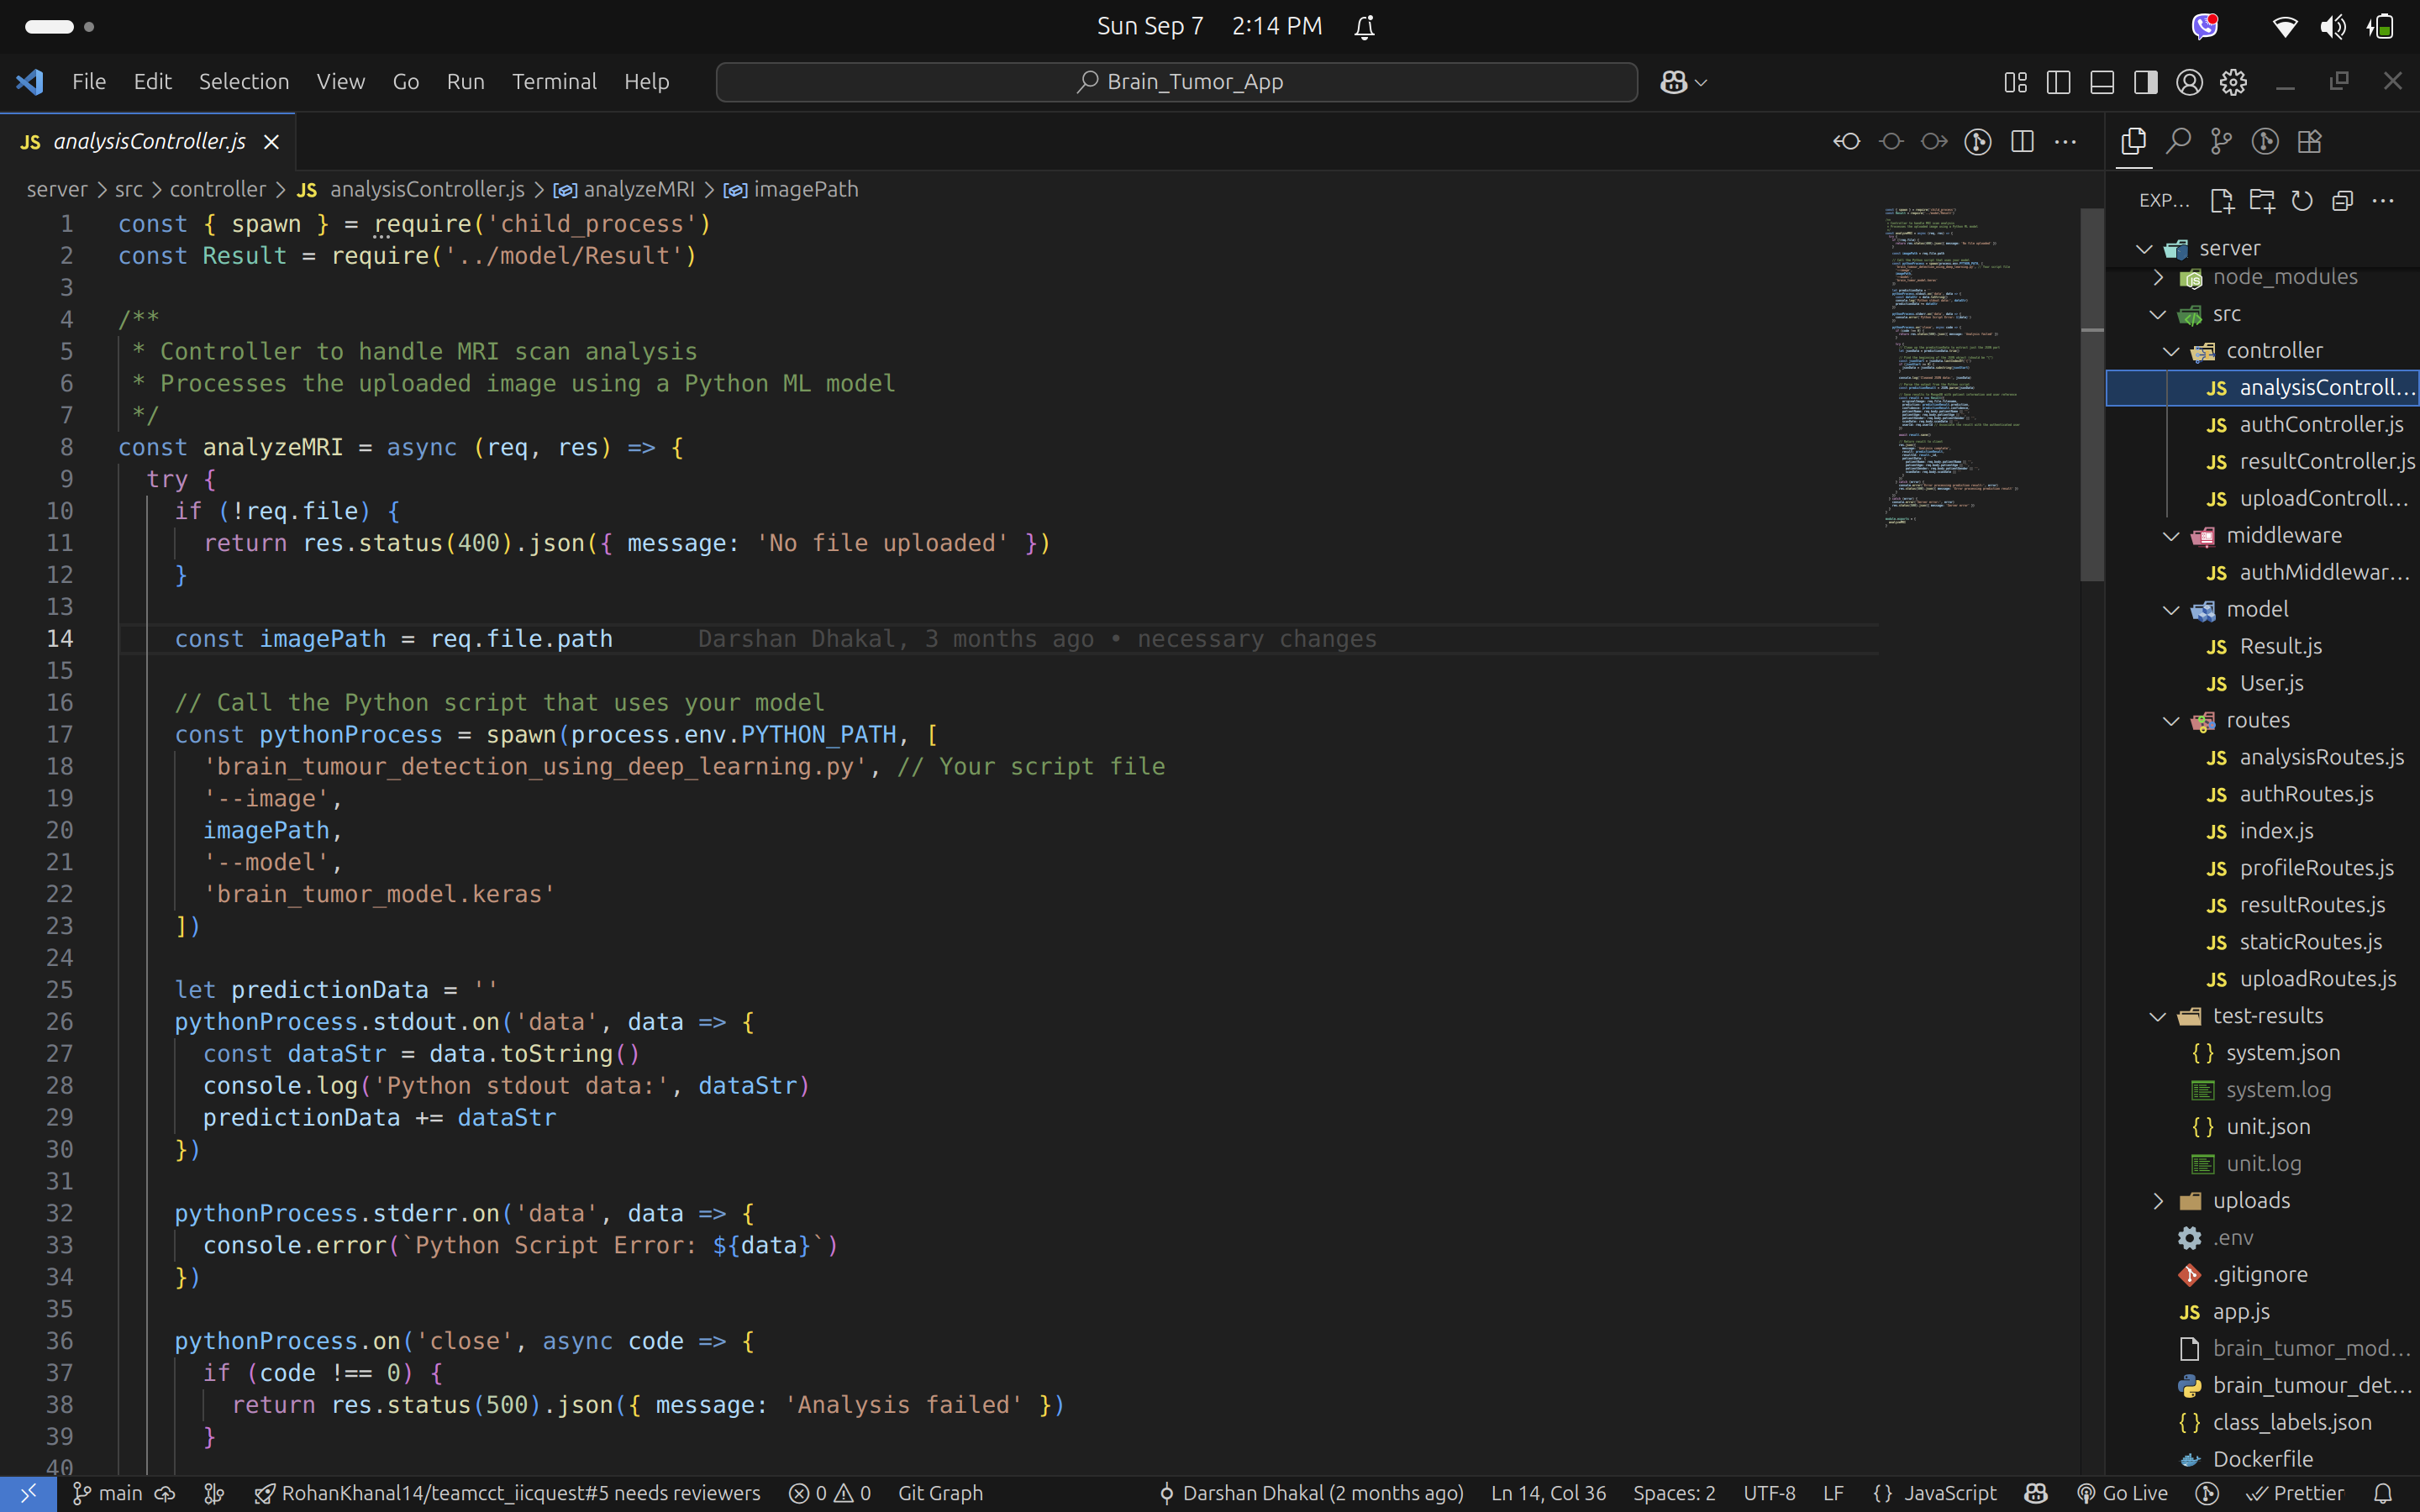
\includegraphics[width=1\linewidth]{App/Backend.png}
    \caption{Backend File Structure of the web application}page of the web application
    \label{fig:backend_page}
\end{figure}

